\documentclass{article}
\usepackage[margin=2cm]{geometry}
\usepackage{tikz}
\usepackage{url}
\begin{document}
\section*{Polar and hexagonal maze profiles}
Created-at: 2026-10-06 14:12 CEST. ETA: 50--70 minutes: profile geometry and
canonical validation, owner tests, Amaterasu generation and physical handoff.

\paragraph{Owner} Formats composes maze descriptions; Core owns IR and semantic
identity; Query reads authored cells/walls; Graph owns weighted spanning-tree
selection and shortest paths; Geometry owns capsule/box collision checks.
No new parser, graph engine, geometry engine or renderer. A separate collaborator
owns physical model composition and the existing MuJoCo/Kawamirai execution.

\paragraph{Profiles} First delivery is a nineteen-cell axial hex maze (radius2;
radius1 remains a small topology test) and a
two-ring, six-sector polar maze. Seeded Graph LCG weights and rank-2 matroid
basis produce connected acyclic passage systems. Hex has six-neighbor topology;
polar has angular and radial neighbors. Explicit boundary segments generate
oriented boxes; circular walls use three facets per sector. The common export
DTO contains cell positions, passages, yaw boxes, endpoints and route points.

\paragraph{Correctness} Canonical source roundtrip and semantic digest;
Query counts and finite field validation; exact geometry/topology consistency;
Graph BFS/Dijkstra distance agreement; seed replay and variation; no passage
through a closed wall. Polar angular moves use intermediate arc points.
Geometry's capsule/box query checks the full route against a 0.85m clearance
radius. This is a geometric corridor witness, not controller success.

\paragraph{Files} Existing example main and visual module; new
\path{hymeko_formats/examples/adversarial_grid/maze.rs}; focused tests in that
module; README; this plan and local report/evidence. The collaborator owns
\path{adversarial_grid/maze_physics.rs}; no overlapping edits there or in physical.rs.
CORE.YAML touched: []. No dependency, public API, schema of old grid or old
physical parameters changed. New profile schema is explicit and versioned.

\paragraph{Bounds} At most 19 profile cells, 72 uncut wall segments, bounded
Graph work. No large campaign or benchmark. Two generated examples, seeds
specified, run on Amaterasu only with fresh output and timeout 180s. Unit tests
are pure and may run locally. Two build jobs; no install, commit/push/merge,
new worktree, Mission Control changes, or implicit simulation.

\paragraph{Risks} Polar chords can cut corners; test full route capsule against
actual faceted walls. Arc joins need overlap. RNG yields a randomized spanning
tree, not a claim of uniformly sampled trees. A provenance mismatch or clearance
failure refuses export. Preserve existing dirty owner work; rollback removes
only this reviewed continuation's delta and leaves prior artifacts unchanged.
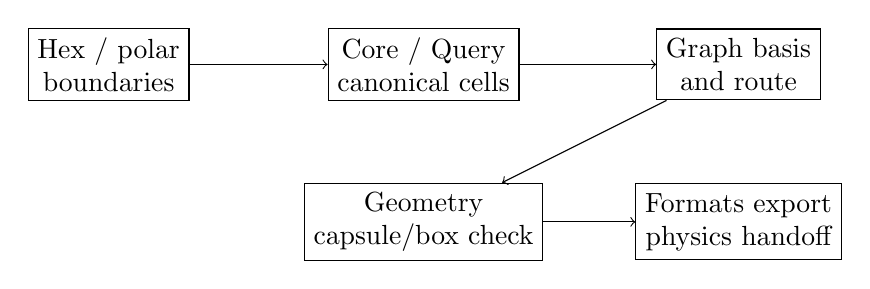
\begin{tikzpicture}[every node/.style={draw,align=center}]
\node (p) at (0,0) {Hex / polar\\boundaries};
\node (ir) at (4,0) {Core / Query\\canonical cells};
\node (g) at (8,0) {Graph basis\\and route};
\node (geom) at (4,-2) {Geometry\\capsule/box check};
\node (exp) at (8,-2) {Formats export\\physics handoff};
\draw[->] (p)--(ir); \draw[->] (ir)--(g); \draw[->] (g)--(geom);
\draw[->] (geom)--(exp);
\end{tikzpicture}

\end{document}
